% Created by tikzDevice version 0.12.6 on 2024-11-13 12:24:00
% !TEX encoding = UTF-8 Unicode
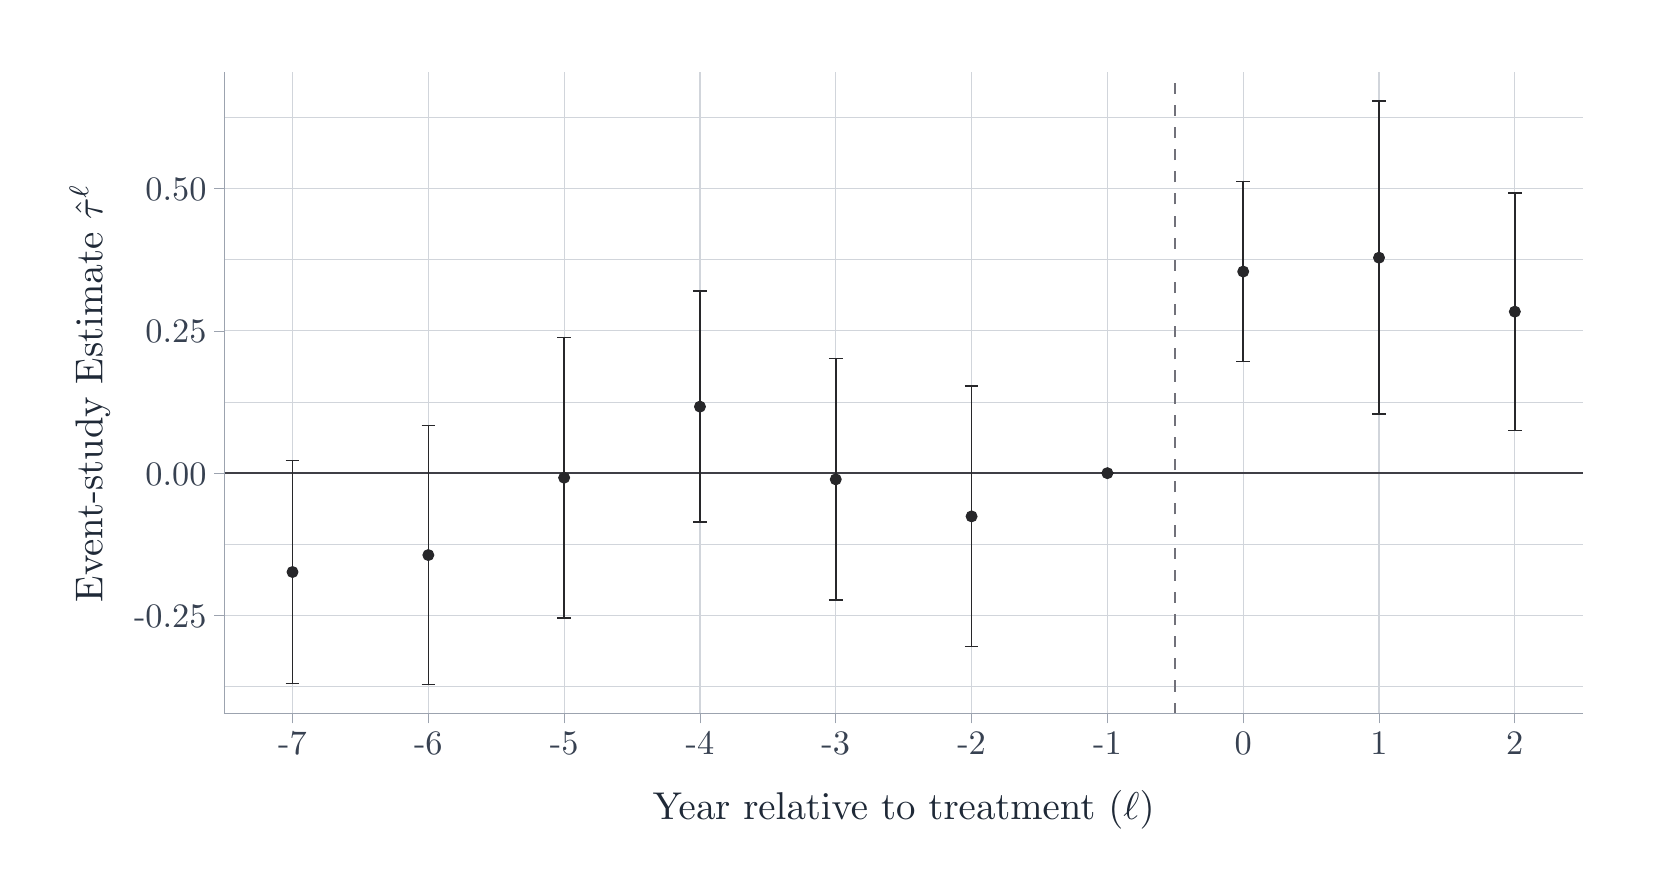
\begin{tikzpicture}[x=1pt,y=1pt]
\definecolor{fillColor}{RGB}{255,255,255}
\path[use as bounding box,fill=fillColor] (0,0) rectangle (578.16,303.53);
\begin{scope}
\path[clip] (  0.00,  0.00) rectangle (578.16,303.53);
\definecolor{drawColor}{RGB}{255,255,255}

\path[draw=drawColor,line width= 0.7pt,line join=round,line cap=round,fill=fillColor] (  0.00,  0.00) rectangle (578.16,303.53);
\end{scope}
\begin{scope}
\path[clip] ( 70.92, 55.65) rectangle (562.16,287.53);
\definecolor{drawColor}{RGB}{255,255,255}
\definecolor{fillColor}{RGB}{255,255,255}

\path[draw=drawColor,line width= 0.7pt,line join=round,line cap=round,fill=fillColor] ( 70.92, 55.65) rectangle (562.16,287.53);
\definecolor{drawColor}{RGB}{209,213,219}

\path[draw=drawColor,line width= 0.4pt,line join=round] ( 70.92, 65.46) --
	(562.16, 65.46);

\path[draw=drawColor,line width= 0.4pt,line join=round] ( 70.92,116.85) --
	(562.16,116.85);

\path[draw=drawColor,line width= 0.4pt,line join=round] ( 70.92,168.24) --
	(562.16,168.24);

\path[draw=drawColor,line width= 0.4pt,line join=round] ( 70.92,219.63) --
	(562.16,219.63);

\path[draw=drawColor,line width= 0.4pt,line join=round] ( 70.92,271.02) --
	(562.16,271.02);

\path[draw=drawColor,line width= 0.4pt,line join=round] ( 70.92, 91.16) --
	(562.16, 91.16);

\path[draw=drawColor,line width= 0.4pt,line join=round] ( 70.92,142.55) --
	(562.16,142.55);

\path[draw=drawColor,line width= 0.4pt,line join=round] ( 70.92,193.94) --
	(562.16,193.94);

\path[draw=drawColor,line width= 0.4pt,line join=round] ( 70.92,245.33) --
	(562.16,245.33);

\path[draw=drawColor,line width= 0.4pt,line join=round] ( 95.70, 55.65) --
	( 95.70,287.53);

\path[draw=drawColor,line width= 0.4pt,line join=round] (144.78, 55.65) --
	(144.78,287.53);

\path[draw=drawColor,line width= 0.4pt,line join=round] (193.85, 55.65) --
	(193.85,287.53);

\path[draw=drawColor,line width= 0.4pt,line join=round] (242.93, 55.65) --
	(242.93,287.53);

\path[draw=drawColor,line width= 0.4pt,line join=round] (292.00, 55.65) --
	(292.00,287.53);

\path[draw=drawColor,line width= 0.4pt,line join=round] (341.08, 55.65) --
	(341.08,287.53);

\path[draw=drawColor,line width= 0.4pt,line join=round] (390.15, 55.65) --
	(390.15,287.53);

\path[draw=drawColor,line width= 0.4pt,line join=round] (439.23, 55.65) --
	(439.23,287.53);

\path[draw=drawColor,line width= 0.4pt,line join=round] (488.30, 55.65) --
	(488.30,287.53);

\path[draw=drawColor,line width= 0.4pt,line join=round] (537.38, 55.65) --
	(537.38,287.53);
\definecolor{drawColor}{RGB}{63,63,70}

\path[draw=drawColor,line width= 0.6pt,line join=round] ( 70.92,142.55) -- (562.16,142.55);
\definecolor{drawColor}{RGB}{113,113,122}

\path[draw=drawColor,line width= 0.6pt,dash pattern=on 4pt off 4pt ,line join=round] (414.69, 55.65) -- (414.69,287.53);
\definecolor{drawColor}{RGB}{39,39,42}
\definecolor{fillColor}{RGB}{39,39,42}

\path[draw=drawColor,line width= 0.4pt,line join=round,line cap=round,fill=fillColor] ( 95.70,106.83) circle (  1.96);

\path[draw=drawColor,line width= 0.4pt,line join=round,line cap=round,fill=fillColor] (144.78,112.96) circle (  1.96);

\path[draw=drawColor,line width= 0.4pt,line join=round,line cap=round,fill=fillColor] (193.85,140.91) circle (  1.96);

\path[draw=drawColor,line width= 0.4pt,line join=round,line cap=round,fill=fillColor] (242.93,166.59) circle (  1.96);

\path[draw=drawColor,line width= 0.4pt,line join=round,line cap=round,fill=fillColor] (292.00,140.31) circle (  1.96);

\path[draw=drawColor,line width= 0.4pt,line join=round,line cap=round,fill=fillColor] (341.08,126.93) circle (  1.96);

\path[draw=drawColor,line width= 0.4pt,line join=round,line cap=round,fill=fillColor] (390.15,142.55) circle (  1.96);

\path[draw=drawColor,line width= 0.4pt,line join=round,line cap=round,fill=fillColor] (439.23,215.40) circle (  1.96);

\path[draw=drawColor,line width= 0.4pt,line join=round,line cap=round,fill=fillColor] (488.30,220.41) circle (  1.96);

\path[draw=drawColor,line width= 0.4pt,line join=round,line cap=round,fill=fillColor] (537.38,200.91) circle (  1.96);

\path[draw=drawColor,line width= 0.6pt,line join=round] ( 93.25,147.13) --
	( 98.16,147.13);

\path[draw=drawColor,line width= 0.6pt,line join=round] ( 95.70,147.13) --
	( 95.70, 66.53);

\path[draw=drawColor,line width= 0.6pt,line join=round] ( 93.25, 66.53) --
	( 98.16, 66.53);

\path[draw=drawColor,line width= 0.6pt,line join=round] (142.32,159.72) --
	(147.23,159.72);

\path[draw=drawColor,line width= 0.6pt,line join=round] (144.78,159.72) --
	(144.78, 66.19);

\path[draw=drawColor,line width= 0.6pt,line join=round] (142.32, 66.19) --
	(147.23, 66.19);

\path[draw=drawColor,line width= 0.6pt,line join=round] (191.40,191.51) --
	(196.31,191.51);

\path[draw=drawColor,line width= 0.6pt,line join=round] (193.85,191.51) --
	(193.85, 90.31);

\path[draw=drawColor,line width= 0.6pt,line join=round] (191.40, 90.31) --
	(196.31, 90.31);

\path[draw=drawColor,line width= 0.6pt,line join=round] (240.47,208.30) --
	(245.38,208.30);

\path[draw=drawColor,line width= 0.6pt,line join=round] (242.93,208.30) --
	(242.93,124.88);

\path[draw=drawColor,line width= 0.6pt,line join=round] (240.47,124.88) --
	(245.38,124.88);

\path[draw=drawColor,line width= 0.6pt,line join=round] (289.55,183.93) --
	(294.46,183.93);

\path[draw=drawColor,line width= 0.6pt,line join=round] (292.00,183.93) --
	(292.00, 96.69);

\path[draw=drawColor,line width= 0.6pt,line join=round] (289.55, 96.69) --
	(294.46, 96.69);

\path[draw=drawColor,line width= 0.6pt,line join=round] (338.62,173.99) --
	(343.53,173.99);

\path[draw=drawColor,line width= 0.6pt,line join=round] (341.08,173.99) --
	(341.08, 79.88);

\path[draw=drawColor,line width= 0.6pt,line join=round] (338.62, 79.88) --
	(343.53, 79.88);

\path[draw=drawColor,line width= 0.6pt,line join=round] (387.70,142.55) --
	(392.61,142.55);

\path[draw=drawColor,line width= 0.6pt,line join=round] (390.15,142.55) --
	(390.15,142.55);

\path[draw=drawColor,line width= 0.6pt,line join=round] (387.70,142.55) --
	(392.61,142.55);

\path[draw=drawColor,line width= 0.6pt,line join=round] (436.77,247.91) --
	(441.68,247.91);

\path[draw=drawColor,line width= 0.6pt,line join=round] (439.23,247.91) --
	(439.23,182.88);

\path[draw=drawColor,line width= 0.6pt,line join=round] (436.77,182.88) --
	(441.68,182.88);

\path[draw=drawColor,line width= 0.6pt,line join=round] (485.85,276.99) --
	(490.76,276.99);

\path[draw=drawColor,line width= 0.6pt,line join=round] (488.30,276.99) --
	(488.30,163.83);

\path[draw=drawColor,line width= 0.6pt,line join=round] (485.85,163.83) --
	(490.76,163.83);

\path[draw=drawColor,line width= 0.6pt,line join=round] (534.92,243.90) --
	(539.83,243.90);

\path[draw=drawColor,line width= 0.6pt,line join=round] (537.38,243.90) --
	(537.38,157.92);

\path[draw=drawColor,line width= 0.6pt,line join=round] (534.92,157.92) --
	(539.83,157.92);
\end{scope}
\begin{scope}
\path[clip] (  0.00,  0.00) rectangle (578.16,303.53);
\definecolor{drawColor}{RGB}{156,163,175}

\path[draw=drawColor,line width= 0.3pt,line join=round] ( 70.92, 55.65) --
	( 70.92,287.53);
\end{scope}
\begin{scope}
\path[clip] (  0.00,  0.00) rectangle (578.16,303.53);
\definecolor{drawColor}{RGB}{55,65,81}

\node[text=drawColor,anchor=base east,inner sep=0pt, outer sep=0pt, scale=  1.24] at ( 64.62, 86.88) {-0.25};

\node[text=drawColor,anchor=base east,inner sep=0pt, outer sep=0pt, scale=  1.24] at ( 64.62,138.27) {0.00};

\node[text=drawColor,anchor=base east,inner sep=0pt, outer sep=0pt, scale=  1.24] at ( 64.62,189.65) {0.25};

\node[text=drawColor,anchor=base east,inner sep=0pt, outer sep=0pt, scale=  1.24] at ( 64.62,241.04) {0.50};
\end{scope}
\begin{scope}
\path[clip] (  0.00,  0.00) rectangle (578.16,303.53);
\definecolor{drawColor}{RGB}{156,163,175}

\path[draw=drawColor,line width= 0.3pt,line join=round] ( 67.42, 91.16) --
	( 70.92, 91.16);

\path[draw=drawColor,line width= 0.3pt,line join=round] ( 67.42,142.55) --
	( 70.92,142.55);

\path[draw=drawColor,line width= 0.3pt,line join=round] ( 67.42,193.94) --
	( 70.92,193.94);

\path[draw=drawColor,line width= 0.3pt,line join=round] ( 67.42,245.33) --
	( 70.92,245.33);
\end{scope}
\begin{scope}
\path[clip] (  0.00,  0.00) rectangle (578.16,303.53);
\definecolor{drawColor}{RGB}{156,163,175}

\path[draw=drawColor,line width= 0.3pt,line join=round] ( 70.92, 55.65) --
	(562.16, 55.65);
\end{scope}
\begin{scope}
\path[clip] (  0.00,  0.00) rectangle (578.16,303.53);
\definecolor{drawColor}{RGB}{156,163,175}

\path[draw=drawColor,line width= 0.3pt,line join=round] ( 95.70, 52.15) --
	( 95.70, 55.65);

\path[draw=drawColor,line width= 0.3pt,line join=round] (144.78, 52.15) --
	(144.78, 55.65);

\path[draw=drawColor,line width= 0.3pt,line join=round] (193.85, 52.15) --
	(193.85, 55.65);

\path[draw=drawColor,line width= 0.3pt,line join=round] (242.93, 52.15) --
	(242.93, 55.65);

\path[draw=drawColor,line width= 0.3pt,line join=round] (292.00, 52.15) --
	(292.00, 55.65);

\path[draw=drawColor,line width= 0.3pt,line join=round] (341.08, 52.15) --
	(341.08, 55.65);

\path[draw=drawColor,line width= 0.3pt,line join=round] (390.15, 52.15) --
	(390.15, 55.65);

\path[draw=drawColor,line width= 0.3pt,line join=round] (439.23, 52.15) --
	(439.23, 55.65);

\path[draw=drawColor,line width= 0.3pt,line join=round] (488.30, 52.15) --
	(488.30, 55.65);

\path[draw=drawColor,line width= 0.3pt,line join=round] (537.38, 52.15) --
	(537.38, 55.65);
\end{scope}
\begin{scope}
\path[clip] (  0.00,  0.00) rectangle (578.16,303.53);
\definecolor{drawColor}{RGB}{55,65,81}

\node[text=drawColor,anchor=base,inner sep=0pt, outer sep=0pt, scale=  1.24] at ( 95.70, 40.78) {-7};

\node[text=drawColor,anchor=base,inner sep=0pt, outer sep=0pt, scale=  1.24] at (144.78, 40.78) {-6};

\node[text=drawColor,anchor=base,inner sep=0pt, outer sep=0pt, scale=  1.24] at (193.85, 40.78) {-5};

\node[text=drawColor,anchor=base,inner sep=0pt, outer sep=0pt, scale=  1.24] at (242.93, 40.78) {-4};

\node[text=drawColor,anchor=base,inner sep=0pt, outer sep=0pt, scale=  1.24] at (292.00, 40.78) {-3};

\node[text=drawColor,anchor=base,inner sep=0pt, outer sep=0pt, scale=  1.24] at (341.08, 40.78) {-2};

\node[text=drawColor,anchor=base,inner sep=0pt, outer sep=0pt, scale=  1.24] at (390.15, 40.78) {-1};

\node[text=drawColor,anchor=base,inner sep=0pt, outer sep=0pt, scale=  1.24] at (439.23, 40.78) {0};

\node[text=drawColor,anchor=base,inner sep=0pt, outer sep=0pt, scale=  1.24] at (488.30, 40.78) {1};

\node[text=drawColor,anchor=base,inner sep=0pt, outer sep=0pt, scale=  1.24] at (537.38, 40.78) {2};
\end{scope}
\begin{scope}
\path[clip] (  0.00,  0.00) rectangle (578.16,303.53);
\definecolor{drawColor}{RGB}{31,41,55}

\node[text=drawColor,anchor=base,inner sep=0pt, outer sep=0pt, scale=  1.40] at (316.54, 17.36) {Year relative to treatment ($\ell$)};
\end{scope}
\begin{scope}
\path[clip] (  0.00,  0.00) rectangle (578.16,303.53);
\definecolor{drawColor}{RGB}{31,41,55}

\node[text=drawColor,rotate= 90.00,anchor=base,inner sep=0pt, outer sep=0pt, scale=  1.40] at ( 27.00,171.59) {Event-study Estimate $\hat{\tau}^{\ell}$};
\end{scope}
\end{tikzpicture}
